\section{Introduction}
\IEEEPARstart{I}{ndustrial-agent} deployments translate task-level goals into
operations over production signals and equipment. A line-speed adjustment,
for example, depends on the active product, recipe, run, applicable limits,
and the control node mapped to the line. If that context changes while a
proposal is awaiting approval, a formerly admissible request may no longer be
appropriate. Device access also needs evidence at two distinct points: what
the command interface reported and what the process was later observed to do.
Connecting these steps across task and device interfaces is therefore a
central industrial integration problem.

Recent work explores end-to-end automation, control-sequence generation,
modular factory skills, and robotic-line control
\cite{xia2025control,huang2026made,koehle2026llmdriven,waseem2026pretrained}.
Other studies address programmable logic controller (PLC) code generation,
context-aware control, resource discovery, shop-floor coordination,
digital-twin fault handling, and natural-language machine access
\cite{liu2026agents4plc,wu2025instructmpc,lim2025llmenabled,zhao2026shopfloor,gill2025llmdt,hofmann2025nlc}.
Recent platforms further connect proposals to Asset Administration Shell
(AAS) models and signed approval, validate actions against process and
instrumentation diagrams (P\&IDs), or organize sensor--manufacturing
execution system (MES)--enterprise resource planning (ERP) evidence streams
\cite{graul2026aas,schall2026safe,lin2026agentic}. Together, these efforts
provide valuable methods for agent reasoning, production context, and
operation constraints.

These studies address complementary aspects of agent operation and motivate an
integration question: how can different task engines and direct calls use a
common operation boundary while accounting for scene-specific devices,
production context, and route-specific evidence? AgentWorkShop addresses this
question through registered harnesses that connect agent engines to task
context and direct representational state transfer (REST) calls that reach the
same named-operation dispatcher. Scene blueprints map semantic signals to
configured drivers and provide targets and guards. The present experiments do
not establish that this design is unique or that all entry paths are equivalent.

Fig.~\ref{fig:control-path} summarizes this control path. Task goals and
production context inform an operation proposal. Shared checks, route guards,
approval when required, and a pre-dispatch context recheck precede writes
through the device write-control (DCW) subsystem. Command receipts and
subsequent data-acquisition (DAQ) observations remain distinct records: a
readback can verify a setpoint, while a later observation describes the
measured process state without, by itself, establishing causation.

\begin{figure}[!b]
\centering
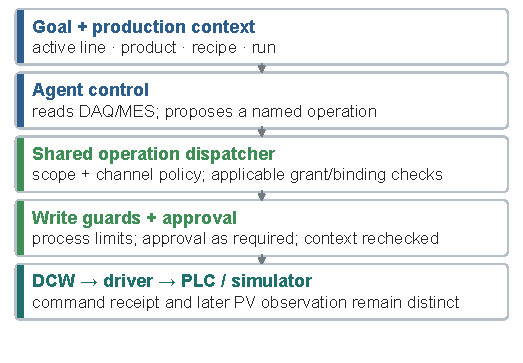
\includegraphics[width=\columnwidth]{resources/fig-agent-control.pdf}
\caption{Agent-control path for a configured industrial task. The agent uses
DAQ and MES context, passes shared operation checks, and routes writes through
process guards, conditional approval, and a pre-dispatch context recheck. DCW
and configured drivers provide device access; command receipts and later
process observations remain separate. Scene configuration supplies targets
and guards, while the application provides its optimization policy.}
\label{fig:control-path}
\end{figure}

AgentWorkShop implements this path as a modular task-to-device framework.
Task requests enter a collaboration runtime whose harness adapters connect
agent engines to production context and available operations. Direct calls
enter the operation dispatcher without creating a task. Scene blueprints and
channel profiles define the signals, objectives, guards, tools, and agent
bindings for a deployment. Fig.~\ref{fig:arch} shows these architectural
relationships, and Fig.~\ref{fig:runtime} follows one registered task through
the execution path.

This paper contributes a modular task-to-device integration design combining a
shared dispatch boundary, scene-specific signal mappings, and separate command
and observation records. Complementary tests examine selected parts of the
design: simulator protocol and node access, entry-specific records, stale
approval-context rejection with a mock driver, and four process missions. In
the component test, every single-field context change was refused before mock
writes; this result concerns the tested approval check, not human review. The
missions trace requests and observations for part weight, film thickness, strip
hardness, and dissolved oxygen. Each scene has one deterministic trajectory,
and no language model selects its setpoints. The checks do not establish
entry-path equivalence, comparative performance, or physical-plant performance.

Section~II reviews related work. Section~III presents the architecture and
execution flow. Section~IV explains the cooperating modules and their device
access and evidence mechanisms. Section~V describes the simulation protocol
and results; Sections~VI and~VII discuss their implications and conclude.
